\documentclass{standalone}
\usepackage{tikz}
\usepackage{tikz-qtree}
\usepackage[makeroom]{cancel}
\usetikzlibrary{fit}


\begin{document} 
	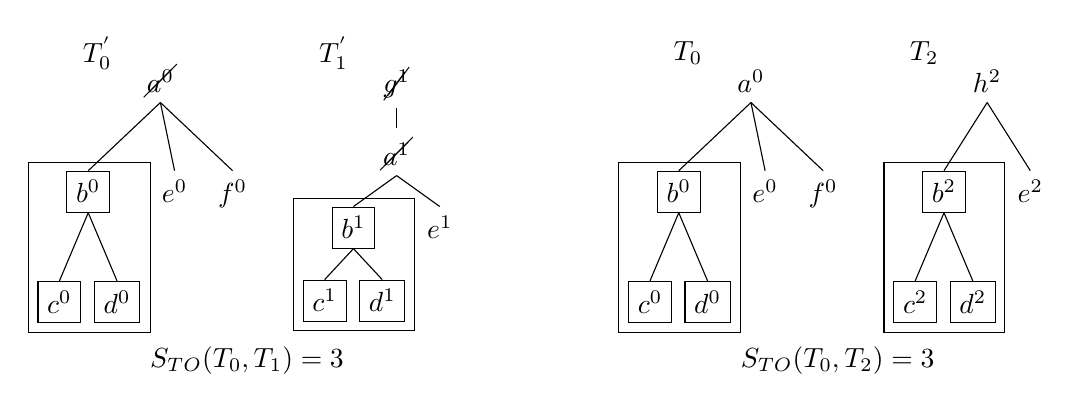
\begin{tikzpicture}[level distance=1.4cm, sibling distance=4.5pt]

	          
		    \node (x) at (-0.8,0.5) {$T_0^{'}$};
		    \node (sto1) at (1.1,-3.4) {$S_{TO}(T_0,T_1) = 3$};
		    \Tree [.\cancel{$a^0$}
		            [.\node[draw]{$b^0$};
		                [.\node(c)[draw]{$c^0$}; ] 
		                [.\node[draw]{$d^0$}; ] 
		            ] 
		            [.$e^0$ ]
		            [.$f^0$ ]
		          ]
		    \node (ph) at (-0.5,-1.25) {\phantom{X}};
		    \node[draw,fit=(c)(ph)]{};
		    

	    \begin{scope}[xshift=3.0cm]
		    \tikzset{level 1+/.style={level distance=2.2\baselineskip}}
			    \node (x) at (-0.8,0.5) {$T_1^{'}$} ;
			    \Tree [.\cancel{$g^1$}
				    	  [.\cancel{$a^1$}
				            [.\node[draw]{$b^1$};
				                [.\node(c)[draw]{$c^1$}; ] 
				                [.\node[draw]{$d^1$}; ] 
				            ] 
				            [.$e^1$ ]
				          ]
				      ]
				\node (ph) at (-0.15,-1.7) {\phantom{X}};
		    	\node[draw,fit=(c)(ph)]{};
	    \end{scope}


	    \begin{scope}[xshift=7.5cm]
		    \node (x) at (-0.8,0.5) {$T_0$};
		    \node (sto1) at (1.1,-3.4) {$S_{TO}(T_0,T_2) = 3$};
		    \Tree [.$a^0$
		            [.\node[draw]{$b^0$};
		                [.\node(c)[draw]{$c^0$}; ] 
		                [.\node[draw]{$d^0$}; ] 
		            ] 
		            [.$e^0$ ]
		            [.$f^0$ ]
		          ]
		    \node (ph) at (-0.51,-1.25) {\phantom{X}};
		    \node[draw,fit=(c)(ph)]{};
	    \end{scope}


	    \begin{scope}[xshift=10.5cm]
			    \node (x) at (-0.8,0.5) {$T_2$} ;
			    \Tree [.$h^2$
				            [.\node[draw]{$b^2$};
				                [.\node(c)[draw]{$c^2$}; ] 
				                [.\node[draw]{$d^2$}; ] 
				            ] 
				            [.$e^2$ ]
				      ]
		    \node (ph) at (-0.15,-1.25) {\phantom{X}};
		    \node[draw,fit=(c)(ph)]{};
	    \end{scope}




	\end{tikzpicture}
\end{document} 